\documentclass[12pt]{article}
\usepackage[utf8]{inputenc}
\usepackage[frenchb]{babel}
\RequirePackage[usenames,dvipsnames,xcolor=pst]{pstricks}
\RequirePackage{epsfig} % for eps fig
\RequirePackage{pst-blur} % for nice shadow
\RequirePackage{pst-dbicons} % for E/R
%\RequirePackage{mon-pst-uml} % for my own UML package
\RequirePackage{pst-uml} % for my own UML package
\RequirePackage{tikz} % circles such as History pseudostate
\newcommand{\monpsgrid}{\psgrid}
%\newcommand{\monpsgrid}{}
\setlength{\topmargin}{-5mm}%
\setlength{\oddsidemargin}{-1mm}%
\setlength{\evensidemargin}{-1mm}%
\setlength{\textwidth}{15.5cm}%
\setlength{\textheight}{8.9in}%
%------------------------------------      
%   QCM
%------------------------------------      
%\usepackage[french,correction]{qcm} % to print correct answers
%\usepackage[french]{qcm}
\title{\vspace{-3pc}\textbf{Contr\^ole M2104--BCOO}}

\date{Jeudi 18 juin 2015 -- Une seule feuille A4 manuscrite autoris\'ee\\
Dur\'ee : 1h30}

\def\dc{\textsf{Diagramme de Classe}}
\def\uc{\textsf{Diagramme de Cas d'Utilisation}}
\def\sni{\textsf{SNI}}
\def\ds{\textsf{Diagramme de S\'equence}}
\def\dss{\textsf{diagramme de S\'equence Syst\`eme}}
%===========================================================
\begin{document}
\maketitle

\section{Liens entre diagrammes}

En utilisant un maximum des éléments de la figure ci-dessous\footnote{Attention, certains diagrammes vous sont inconnus et ne sont donc pas à utiliser.}, placez-les dans un schéma
en indiquant les liens de dépendances entre eux.

\scalebox{0.6}{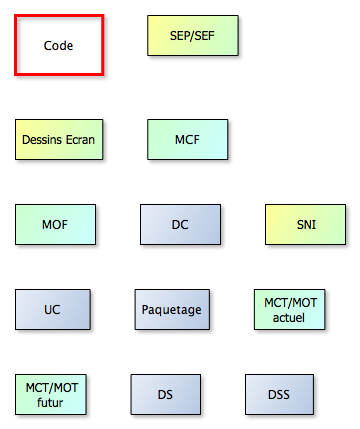
\includegraphics{fig-enchainement-sujet}}

\section{Rétro-conception}

\subsection*{Sujet}

Vous intervenez en support à un projet où le code fonctionne
mais où les développeurs sont partis avec presque tous les documents et ont volontairement enlevé tous les commentaires utiles de leur code\footnote{Le sujet est fictif mais le code et les diagrammes proviennent d'une réalisation réelle d'étudiants de 2ème année du DUT, promo 2014.}.

Il ne reste que le \uc{} et le \sni{} ci-dessous :

\scalebox{0.5}{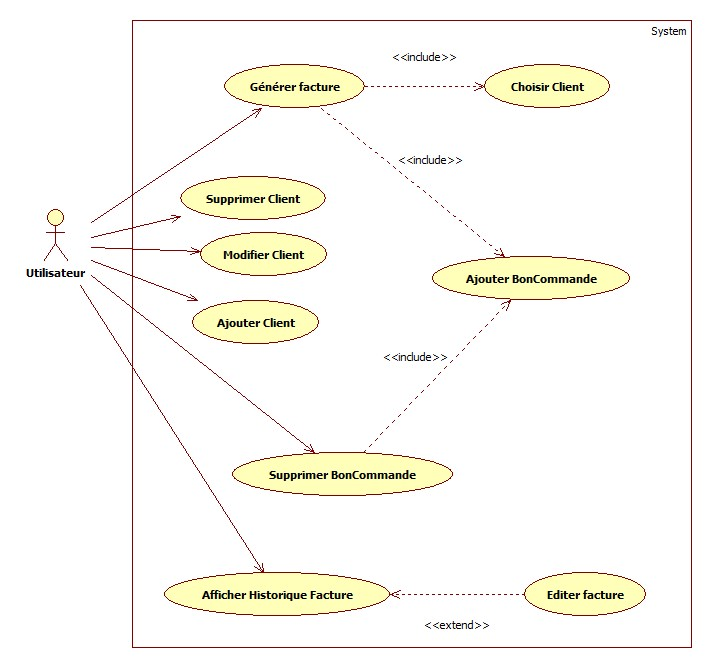
\includegraphics{exam-uc}}

\scalebox{0.5}{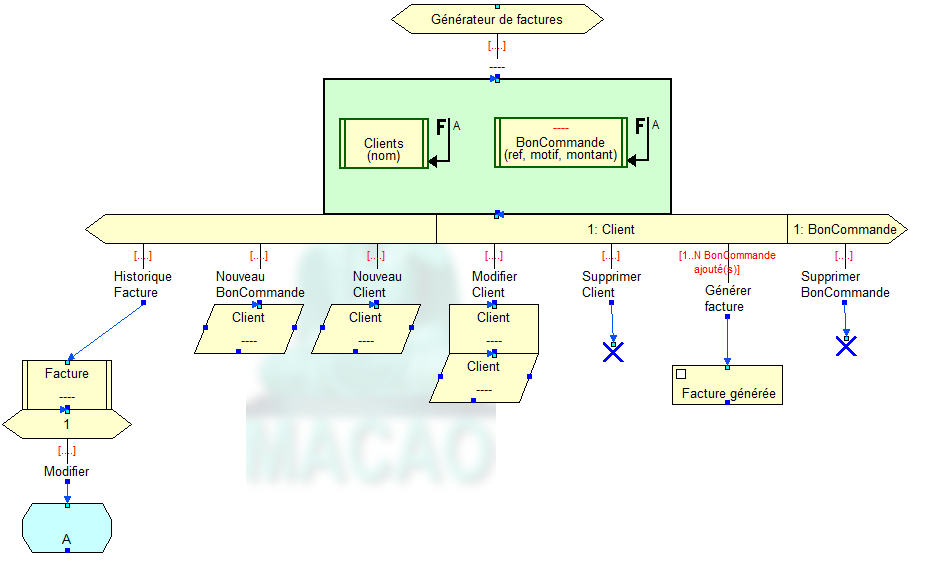
\includegraphics{exam-sni}}

\subsection{Diagramme de classe}

En vous inspirant du code fournit en annexe, réalisez le \dc{} correspondant en intégrant les classes métiers, de vue, et de contrôle. Vous veillerez à faire apparaître les dépendances et les associations\footnote{Vous pouvez réaliser plusieurs diagrammes de classes pour plus de lisibilité, du moment qu'ils sont cohérents et complémentaires.}.

\subsection{Diagramme de séquence}

Quand on clique sur le bouton "Nouveau" du menu principal, on obtient :

\scalebox{0.4}{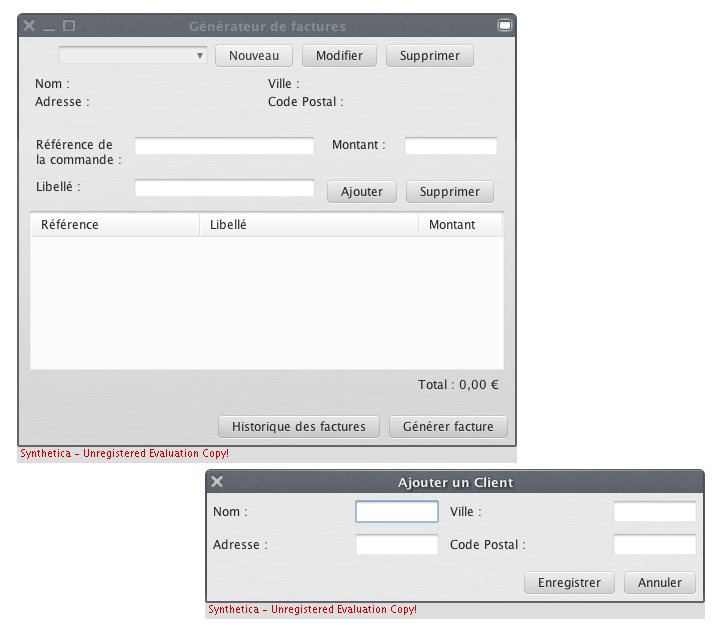
\includegraphics{exam-prodif}}

En vous inspirant des éléments en votre possession, réalisez le \ds{} du cas \texttt{Ajouter Client}. On fera le scénario nominal, c'est à dire sans erreur de saisie, etc. On démarrera le scénario à la fenêtre dédiée à ce cas d'utilisation (\texttt{Ajouter Client}). 

\subsection{Diagramme d'architecture MVC}

Proposez un diagramme des paquetages MVC avec les classes (sans méthodes ni attributs
ni associations),  et les dépendances.

\section{Questionnaire à Choix Multiple}

Réalisez le QCM distribué à part et rendez-le avec votre copie (après y avoir inscrit votre nom).

\newpage
\section*{Bar\`eme prévisionnel}

\begin{description}
\item[1] 2 points 
\item[2.1] 2 points 
\item[2.2] 4 points 
\item[2.2] 2 points 
\item[3] 10 points 
\end{description}

\end{document}
%===========================================================